\documentclass[11pt]{article}

\makeatletter
\def\s@btitle{\relax}
\def\subtitle#1{\gdef\s@btitle{#1}}
\def\@maketitle{%
  \newpage
  \null
  \vskip 2em%
  \begin{center}%
  \let \footnote \thanks
    {\LARGE \@title \par}%
                \if\s@btitle\relax
                \else\typeout{[subtitle]}%
                        \vskip .5pc
                        \begin{large}%
                                \textsl{\s@btitle}%
                                \par
                        \end{large}%
                \fi
    \vskip 1.5em%
    {\large
      \lineskip .5em%
      \begin{tabular}[t]{c}%
        \@author
      \end{tabular}\par}%
    \vskip 1em%
    {\large \@date}%
  \end{center}%
  \par
  \vskip 1.5em}
\makeatother


\newcommand{\todo}[1]{{\bf ??? #1 ???}}
\usepackage{a4wide}
%\usepackage{psfig}
\usepackage{amssymb}
\usepackage{algorithm,algorithmic,amstext}
%\usepackage{showkeys}
%\usepackage{epsfig}
\usepackage{url}
\usepackage{color}
\usepackage{graphicx}

\newcommand{\sq}[4]{\left[\begin{array}{cc}#1&#2\\#3&#4\end{array}\right]}
\newcommand{\flax}[2]{\left[\begin{array}{c}#1\\#2\end{array}\right]}
\newcommand{\flay}[2]{\left[\begin{array}{cc}#1&#2\end{array}\right]}
\newcommand{\fltt}[1]{\left[\begin{array}{cc}#1_{11}&#1_{12}\\#1_{21}&#1_{22}\end{array}\right]}
\newcommand{\flot}[1]{\left[\begin{array}{cc}#1_{1}&#1_{2}\end{array}\right]}
\newcommand{\flto}[1]{\left[\begin{array}{c}#1_{1}\\#1_{2}\end{array}\right]}
\newcommand{\hide}[1]{}
\newcommand {\algcodecost}      [3]  {\ind{#1}\codesize$ #2 $\>\codesize$#3$\\[-0.1cm]}
\newcommand{\R}{{\mathbb R}}
%%%%%%%%%%%%%%%%%%%%%%%%%%%%%%%%%%%%%%%%%%%%%%%%%%%%%%%%%%%%%%%%%%%%%%%%
%
% Make @ act like a letter, temporarily, in order to access
% internal control sequences of plain format.
\catcode`@=11
%
% hacked border matrix macro
\font\tenex=cmex10 % math extension
\newdimen\p@renwd
\setbox0=\hbox{\tenex B} \p@renwd=\wd0 % width of the big left [
\def\bmat#1{\begingroup \m@th
  \setbox\z@\vbox{\def\cr{\crcr\noalign{\kern2\p@\global\let\cr\endline}}%
    \ialign{$##$\hfil\kern2\p@\kern\p@renwd&\thinspace\hfil$##$\hfil
      &&\quad\hfil$##$\hfil\crcr
      \omit\strut\hfil\crcr\noalign{\kern-\baselineskip}%
      #1\crcr\omit\strut\cr}}%
  \setbox\tw@\vbox{\unvcopy\z@\global\setbox\@ne\lastbox}%
  \setbox\tw@\hbox{\unhbox\@ne\unskip\global\setbox\@ne\lastbox}%
  \setbox\tw@\hbox{$\kern\wd\@ne\kern-\p@renwd\left[\kern-\wd\@ne
    \global\setbox\@ne\vbox{\box\@ne\kern2\p@}%
    \vcenter{\kern-\ht\@ne\unvbox\z@\kern-\baselineskip}\,\right]$}%
  \null\;\vbox{\kern\ht\@ne\box\tw@}\endgroup}
%
% @ is no longer a letter
\catcode`@=12

\begin{document}

\title{SCASY Users' Guide\thanks{
{\bf Technical Report UMINF-09.10.} This research was conducted using
the resources of the High Performance Computing Center North
(HPC2N). Financial support has been provided by the \emph{Swedish
Research Council} under grant VR 70625701  and by the
\emph{Swedish Foundation for Strategic Research} under grant A3
02:128. }}

\subtitle{Release 1.0}

\author{\renewcommand{\thefootnote}{\arabic{footnote}}
Robert Granat and Bo K{\aa}gstr{\"{o}}m\footnotemark[1]}

\footnotetext[1]{Department of Computing Science and HPC2N,
Ume{\aa} University, SE-901 87 Ume\aa, Sweden. E-mail: {\tt
\{granat,bokg\}@cs.umu.se}}

\date{\today.}
\maketitle

\begin{abstract}
\noindent The functionality, the contents, some implementation issues, and the
proper usage of the latest release of the SCASY software library are presented. 

%\end{abstract}

\vspace{5mm}
%
\noindent {\bf Keywords:} SCASY, parallel software, ScaLAPACK,
Sylvester-type matrix equations
\end{abstract}

\pagenumbering{arabic}

\section{Introduction}
\label{sec:introduction} The SCASY library is a high performance
software library for solving Sylvester-type matrix equations on
distributed memory platforms. The focus of SCASY is on robustness,
speed and scalability (see also the ACM TOMS Algorithms Policy \cite{ACMAlgPolicy}). 
This SCASY Users' Guide is a supplement to the 
ACM Transactions on Mathematical Software articles 
\cite{granatkagstrom09a,granatkagstrom09b}.

\section{Algorithms for Sylvester-type matrix equations} \label{sec:algorithms}
In this section, we give a brief overview of the algorithms
underlying the implementations available through SCASY.

The algorithms in SCASY for Sylvester-type matrix equations are
presented in \cite{granatkagstrom09a,granatkagstrom09b} and in the
technical reports \cite{granatkagstrom07a,granatkagstrom07b}.
Table \ref{tab:matrixequations} summarizes the considered
Sylvester-type matrix equations.

\begin{table}[!htb]
\centering \small
\begin{tabular}{|l|l|l|} \hline
~Name & Matrix Equation & Acronym \\ \hline
~Standard CT Sylvester& ${\rm op}(A)X \pm X{\rm op}(B)   = sC \in \R^{m\times n}$ & SYCT \\
~Standard DT Lyapunov   & ${\rm op}(A)X  +  X{\rm op}(A^T) = sC \in \R^{m\times m}$ & LYCT \\
~Standard DT Sylvester & ${\rm op}(A)X{\rm op}(B) \pm X   = sC \in \R^{m\times n}$ & SYDT \\
~Standard DT Lyapunov  & ${\rm op}(A)X{\rm op}(A^T) - X   =sC \in \R^{m\times m}$ & LYDT \\
$\begin{array}{l}\mbox{Generalized Coupled} \\ \mbox{Sylvester}
\end{array}$
 &
    $ \left\{ \begin{array}{c}
    {\rm op}(A)X \pm Y {\rm op}(B) = sC \in \R^{m\times n} \\
    {\rm op}(D)X \pm Y {\rm op}(E) = sF \in \R^{m\times n} \\
    \end{array} \right. $ & GCSY \\
~Generalized Sylvester   & ${\rm op}(A)X{\rm op}(B) \pm {\rm
op}(C)X{\rm op}(D)=sE \in \R^{m\times n}$
& GSYL \\
~Generalized CT Lyapunov & ${\rm op}(A)X{\rm op}(E^T)+{\rm
op}(E)X{\rm op}(A^T)=sC \in \R^{m\times m}$
& GLYCT \\
~Generalized DT Lyapunov & ${\rm op}(A)X{\rm op}(A^T)-{\rm
op}(E)X{\rm op}(E^T)=sC \in \R^{m\times m}$
& GLYDT \\
\hline
\end{tabular}
\caption{Sign and transpose variants of the Sylvester-type matrix
equations considered in SCASY. CT and DT denote the
continuous-time and discrete-time variants, respectively. The
scalar $s$, where $0 < s \leq 1.0$, is a scaling factor used to
prevent from overflow in the solution process.}
\label{tab:matrixequations}
\end{table}

The algorithms are based on the classical Bartels--Stewart's
method \cite{bartelsstewart72} which utilizes standard and
generalized Schur decompositions (see, e.g.,
\cite{golubvanloan96}) to reduce the matrix equations into a
triangular Schur form. These reduced matrix equations are solved using
combined forward- and backward substitution techniques. For
illustration, consider SYCT:
%
\begin{itemize}
\item Transform $A$ and $B$ to real Schur form (see, e.g.,
\cite{golubvanloan96}), i.e., compute the factorizations $T_A
=Q^TAQ$ and $T_B=P^TBP$, where $Q \in \mathbb{R}^{m \times m}$ and
$P \in \mathbb{R}^{n \times n}$ are orthogonal and $T_A$ and $T_B$
are upper quasi-triangular, i.e., having $1 \times 1$ and $2
\times 2$ diagonal blocks corresponding to real and complex
conjugate pairs of eigenvalues, respectively. \item Update $C$
with respect to the Schur decompositions by the two-sided
transformation $\tilde{C}=Q^TCP$. \item Solve the resulting
reduced triangular matrix equation for the intermediate solution
matrix $\tilde{X}$, see below. \item Transform the intermediate
solution back to the original coordinate system by a second
two-sided transformation $X=Q\tilde{X}P^T$.
\end{itemize}
%
The triangular matrix equation is solved by several layers of
explicit and/or recursive blocking, leading to algorithms which
are very rich in GEMM-updates in the right hand side(s); on the
leaf nodes of the blocking, we consider small-sized matrix
equations in an equivalent linear systems of equations $Zx=y$,
where $Z=I_{n} \otimes A - B^T \otimes I_{m}$ is a Kronecker
product representation of the corresponding Sylvester-type
operator ($AX-XB$ for SYCT). This reformulation is also the key observation which
enables condition estimation using the technique developed in
\cite{hager84,higham88,kagstromporomaa92}. \\\

%\subsection{Algorithms for eigenvalue reordering}
%\label{sec:reord} Given a general square matrix $A \in
%\mathbb{R}^{n \times n}$, the Schur decomposition
%%
%\begin{equation}
%\label{eq:schur0}
%    Q^TAQ = T
%\end{equation}
%%
%is the standard approach to solving {non-symmetric eigenvalue
%problems, that is, computing eigenvalues and invariant subspaces
%(or eigenvectors) of a general dense matrix. In Equation
%(\ref{eq:schur0}), $T \in \mathbb{R}^{n \times n}$ is
%quasi-triangular with diagonal blocks of size $1 \times 1$ and $2
%\times 2$ corresponding to real and complex conjugate pairs of
%eigenvalues, respectively, and $Q \in \mathbb{R}^{n \times n}$ is
%orthogonal. For any decomposition of (\ref{eq:schur0}) in the form
%%
%\begin{equation}
%\label{eq:schur}
%    Q^TAQ = T \equiv
%        \left[ \begin{array}{cc}
%        T_{11} & T_{12} \\
%           0    & T_{22} \\
%        \end{array} \right]
%\end{equation}
%%
%with $T_{11} \in \mathbb{R}^{p \times p}$ for some integer $p$,
%the first $p$ columns of the matrix $Q$ span an {\em invariant
%subspace} of $A$ corresponding to the $p$ eigenvalues of $T_{11}$.
%Invariant subspaces are an important generalization of
%eigenvectors and often eliminate the need for calculating a
%potentially ill-conditioned set of eigenvectors in applications.
%
%When applying the QR algorithm for computing a Schur form, one has
%little influence on the order of the eigenvalues on the diagonal.
%For computing an invariant subspace with specified eigenvalues,
%they must belong contained to the block $T_{11}$
%of~(\ref{eq:schur}). For example, in applications related to
%dynamical systems and control, it is often desired to compute the
%stable invariant subspace, in which case $T_{11}$ is to contain
%all eigenvalues of $A$ that have negative real part. To achieve
%this goal, the output of the QR algorithm needs to be
%post-processed by {\em eigenvalue reordering}.
%
%Bai and Demmel proposed a direct algorithm for reordering adjacent
%eigenvalues in the real Schur form \cite{baidemmel93} to attain
%such invariant subspaces. Kressner developed a block version of
%this algorithm \cite{kressner04a}, which substantially improved
%its efficiency on architectures with deep memory hierarchies by
%reordering several eigenvalues simultaneously instead of
%reordering each eigenvalue individually. In this release of SCASY,
%we include a parallel blocked variant of the blocked algorithm for
%eigenvalue reordering in the real standard and generalized Schur
%forms that were presented in \cite{granatkagstromkressner09d}.
%Those algorithms are used in parallel computation of invariant and
%deflating subspaces corresponding to specified sets of
%eigenvalues, e.g.,
%stable subspaces in linear-quadratic optimal control ~\cite{Meh91}.\\\
%
%\noindent {\bf Main contributors:} Robert Granat, Bo
%K{\aa}gstr{\"{o}}m, and Daniel Kressner.
%
%\subsection{Algorithms for Riccati-type matrix equations}
%\label{sec:riccati} The continuous-time algebraic Riccati equation
%(CARE) is defined as
%\begin{equation} \label{eq:care}
%0 = Q + A^T X + XA - XBR^{-1}B^TX,
%\end{equation}
%with $A \in \R^{n\times n}$, $Q \in \R^{n\times n}$ symmetric
%positive semi-definite, $R \in \R^{m \times m}$ symmetric
%non-singular, $B \in \R^{n \times m}$ and the solution matrix $X
%\in \R^{n\times n}$. A highly performing implementation of the a
%Schur-based CARE solver based on parallel eigenvalue reordering
%and the existing ScaLAPACK \cite{slug,blackfordetal97} Schur
%decomposition was presented in \cite{granatkagstromkressner08}.
%The software was extended to include also the discrete-time
%algebraic Riccati equations (DAREs) of the form
%%
%\begin{equation} \label{eq:dare}
%    X = A^T X A - A^T X B (R + B^T X B)^{-1}  B^T X A + Q.
%\end{equation}
%%
%
%With $G = BR^{-1}B^T$, the CARE (\ref{eq:care}) is solved by
%constructing the Hamiltonian matrix
%\begin{equation} \label{eq:CARE_Hamiltonian}
%    H_{\rm CARE} = \left[ \begin{array}{cc}
%        A & G \\
%        Q & -A^T
%    \end{array} \right].
%\end{equation}
%Under mild conditions, the $2n\times 2n$ matrix $H_{\rm CARE}$ has
%$n$ stable eigenvalues. If $\big[{X_1 \atop X_2} \big]$ with
%$X_1,X_2\in \R^{n\times n}$ denotes a basis for the invariant
%subspace belonging to these eigenvalues then $X_1$ is invertible
%and $X = -X_2 X_1^{-1} \in \R^{n\times n}$ is the stabilizing
%solution of CARE.
%
%With $A$ non-singular, the DARE is solved by computing an
%invariant subspace of any of the Hamiltonian matrices
%%
%\begin{equation} \label{eq:DARE_Hamiltonian1}
%    H{_{\rm DARE}}_1 = \left[ \begin{array}{cc}
%        A^{-1} & A^{-1}G \\
%        QA^{-1} & A^T + QA^{-1}G
%    \end{array} \right]
%\end{equation}
%and
%\begin{equation} \label{eq:DARE_Hamiltonian2}
%    H{_{\rm DARE}}_2 = \left[ \begin{array}{cc}
%        A^{-1} & A^{-1}G \\
%        QA^{-1} & A^T + QA^{-1}G
%    \end{array} \right],
%\end{equation}
%%
%similarly to the CARE case.
%
%Notice that for the case of parallel software for Riccati-style
%matrix equations, SCASY only provides \emph{preliminary
%proof-of-concept academic implementations}, which are not well
%tested. \\\
%
%\noindent {\bf Main contributors:} Robert Granat, Bo
%K{\aa}gstr{\"{o}}m, and Daniel Kressner.
%
%\subsection{Algorithms for real Schur decompositions - parallel QR/QZ algorithms}
%\label{sec:schur} The Schur decomposition (\ref{eq:schur0}) is the
%first step in numerical computation of eigenspaces with specified
%eigenvalues. The standard procedure for computing the Schur form
%is the QR algorithm (see, e.g., \cite{golubvanloan96}).
%
%New algorithms and implementations for the parallel QR algorithm
%was presented in \cite{granatkagstromkressner09} and a preliminary
%version is included in the current release of SCASY. This
%compilation of software provides efficient parallel computation of
%invariant subspaces, which reduces TTD ({\em
%Total-Time-to-Delivery}) for Schur-based algorithms in numerical
%linear algebra, e.g., Laub's method for solving Riccati matrix
%equations \cite{laub79}.
%
%The generalized Schur decomposition
%%
%\begin{equation}
%    (S,T) = Q^T (A,B) Z,
%\end{equation}
%%
%where $(A,B)$ is a regular matrix pair, $Q$ and $Z$ are orthogonal
%matrices and $(S,T)$ is the generalized real Schur form (see,
%e.g., \cite{golubvanloan96}) plays an analogous role in numerical
%methods for matrix pairs and is preferably computed using the QZ
%algorithm, e.g, in Bartels--Stewart-style methods for solving
%generalized Sylvester-type matrix equations (see Section
%\ref{sec:algorithms}}. Parallel algorithms for the implementation
%of the generalized Hessenberg-triangular reduction and the QZ
%algorithm was presented in
%\cite{adlerborndacklandkagstrom02,adlerbornkagstromkressner06}
%and prototype implementations are included in the SCASY package. \\\
%
%The plan is to contribute these algorithms to ScaLAPACK when they
%have reached production code quality.
%
%\noindent {\bf Main contributors:} Bj{\"{o}}rn Adlerborn, Robert
%Granat, Bo K{\aa}gstr{\"{o}}m and Daniel Kressner.

\section{Software} \label{sec:software}
In this section, we present the parallel software that implements
the SCASY algorithms.

\subsection{Implementation notes}
The algorithms in SCASY are implemented using Fortran 90/95
following the coding conventions that are typical for LAPACK
\cite{lapack3} and ScaLAPACK \cite{blackfordetal97}. The
underlying parallel computing paradigm follows the ScaLAPACK standard:
%
\begin{itemize}
    \item The parallel processes are organized into a
    rectangular $P_r \times P_c$ mesh labelled from $(0,0)$
    to $(P_r-1,P_c-1)$ according to their specific position
    indices in the mesh.
    \item The matrices are distributed over the mesh using
    2-dimensional (2D) block cyclic mapping with the block
    sizes $m_b$ and $n_b$ in the row and
    column dimensions, respectively, i.e. each distributed block
    is of size $m_b \times n_b$.
\end{itemize}
%
The codes in the SCASY package have been tested extensively with
the Portland Group Compiler suite and the Pathscale Compiler
suite, and also with the GNU Fortran compiler and the NAG
Fortran Compiler.

\subsection{Download location}
\label{sec:download} The stable version of SCASY published for ACM TOMS
is available on CALGO \cite{CALGO}. Other SCASY releases (including bug-fixes and new features) are available via the library homepage \cite{scasy} in either {\tt .zip} or {\tt
.tar.gz} format with the name \texttt{scasy\_latest}. The latest version can also
be retrieved via correspondence with the authors.

\subsection{Library installation} \label{sec:usage}
In what follows, we assume that the user works in a Linux-like
environment and has downloaded the latest SCASY release in the
{\tt .tar.gz} format. (The software package has the same structure
in the {.zip} format, but the accompanying Makefiles are most
likely irrelevant in a Windows-like environment.)

Note that there is currently no installation routine; after the
library has been built, it should be moved to a proper location
(e.g., \texttt{/usr/local/lib}).

\subsubsection{A look inside the SCASY tar-ball}
To unpack the tar-ball, move to a proper working directory and try
%
\begin{verbatim}
host:~> tar zxvf scasy_latest.tar.gz
\end{verbatim}
%
to unpack the library. This will reveal the SCASY root directory,
which is called \texttt{scasy[x.y]}, where \texttt{[x.y]} denotes
the current release and version numbers\footnote{Current release
is 1.0.}. Inside this root directory, the \texttt{ls} command will
reveal the following files and directories:
%
\begin{verbatim}
docs/ lib/ make/ Makefile Make_include README test/.
\end{verbatim}
%
In what follows, we give an overview of the interior of each item
above:

\begin{description}
    \item[\texttt{docs/}] This directory contains the
    documentation necessary to understand how to install and use
    the SCASY library, e.g., the latest version of this Users'
    Guide \cite{sug} as well some material related to the SCASY
    homepage \cite{scasy}.
    \item[\texttt{lib/}] This directory contains all the Fortran
    source code as \texttt{.f} files (which implies that explicit
    pre-processing is necessary, see Section
    \ref{sec:preprocess}), and a few C (\texttt{.c}) files which are
    compiled and attached
    to the library; these files are used mostly for debugging purposes
    and most users can ignore them, as long as a proper C compiler
    is chosen. The directory also includes a local
    \texttt{Makefile} which compiles and builds the library via a
    call from the root directory \texttt{Makefile} (which is described
    below). The library will also be built in this directory as the archive \texttt{libscasy.a}.
    \item[\texttt{make/}] For the user's convenience, this directory contains
    template \texttt{Make\_include} files (see below) which are specific to each of the
    following compilers: Portland Group, Pathscale, GNU Fortran
    and NAG Fortran Compiler.
    \item[\texttt{Makefile}] This \texttt{Makefile} is responsible
    for building the library and the attached test program (see
    below) from the root directory, when called by the user.
    \item[\texttt{Make\_include}] In principle, \emph{this file is the
    only one the user needs to modify} to build the library and the
    attached test program correctly. By using the available
    templates, see above, the modification can be carried out
    easily. Necessary modifications include choice of Fortran (and C) compilers,
    the associated Fortran compiler flags (the C compiler only uses \texttt{-c}),
    pre-processing options (see below), linking options, paths to external libraries, etc.
    \item[\texttt{README}] This file contains some information
    quite similar to this Users' Guide, but is much shorter and
    serves more like a Quick Start Guide to the library.
    \item[\texttt{test/}] This directory contains the Fortran file
    \texttt{TESTSCASY.f} and another local \texttt{Makefile},
    which is responsible for compiling and linking the test
    program with the library. We give more information on the
    usage of the test program in Section \ref{sec:testprogram}.
\end{description}

\subsubsection{Pre-processing options}
\label{sec:preprocess} The following pre-processing options are
available for the SCASY library:
%
\begin{description}
    \item[\texttt{USE\_DYNAMIC}] When this option is activated, the test program uses dynamic
allocation (which is recommended). If this option is not
activated, all allocations are done statically in the test
program.

\item[\texttt{USE\_INTEGER8}] When this option is activated, the
test program uses 8 byte integers to specify the size of the
memory areas to be allocated (recommended, especially in cases
when large matrices are considered).

\item[\texttt{LOOPGRID}] When this option is activated, the test
program loops through the possible process grid dimensions
specified by its local variables \texttt{[ACRO]\_NPROW\_MIN},
\texttt{[ACRO]\_NPROW\_MAX}, \texttt{[ACRO]\_NPCOL\_MIN},
\texttt{[ACRO]\_NPCOL\_MAX} using the step variables
\texttt{[ACRO]\_NPROW\_STEP} and \texttt{[ACRO]\_NPCOL\_STEP}. The
user is responsible for allocating enough MPI processes when
executing the test program such that
\begin{verbatim}
    # MPI processes >= [ACRO]_NPROW_MAX*[ACRO]_NPCOL_MAX
\end{verbatim}
otherwise the test program will abort with an error message. If
this option is not activated, the test program ignores the
specified process grid dimensions listed above and simply creates
an "as-square-as-possible" rectangular process grid such that
\texttt{NPROW*NPCOL} is as close to the number of allocated MPI
processes as possible.

\item[\texttt{USE\_OMP}] When this option is activated, both the
library and the test program expand OpenMP directives for building
an application that can be executed in a distributed memory
environment with multi-threaded nodes. The number of nodes in the
process grid is specified as usual by allocating a number of MPI
processes in combination with/without the \texttt{LOOPGRID}
option. The number of threads per node is specified by the
environment variable \texttt{OMP\_NUM\_THREADS}.

\item[\texttt{USE\_NEWPQR}] When this option is activated, the
current ScaLAPACK implementation of the unsymmetric QR algorithm
is replaced with a new preliminary multishift version with
advanced deflation techniques (see \cite{granatkagstromkressner09}
for some preliminary results), which should give the general
solvers for the standard equations a considerable speed boost.

\item[\texttt{USE\_AED\_RES}] When this option is activated
together with \texttt{USE\_NEWPQR}, the new parallel QR algorithm
used in SCASY checks the residual of each Schur decomposition
computed in each stage of aggressive early deflation and saves the
maximum results to an output array. This option is mostly used for
debugging purposes, and is not recommended for non-expert users.
\end{description}
%
We remark that these pre-processing options are included in the
template \texttt{Make\_include} files for the convenience of the
user.

\subsubsection{How to use the attached test program}
\label{sec:testprogram} Detailed instructions on how to use the
attached test program are given in the 736 first lines of the
corresponding source file \texttt{test/TESTSCASY.f}. By default,
the program is tuned for testing all driver routines listed in
Table \ref{tab:routines} in sequence for matrices of size $2048$,
and when \texttt{LOOPGRID} is defined it will be using up to $4$
MPI processes. From a user's point of view, the attached test
program could be considered as a starting point for a simple
installation test. From portability aspects across different
parallel systems, the authors have refrained from making this
test automatic.

As long as the user allocates the correct number of
MPI processes with {\tt mpiexec} or {\tt mpirun} (or equivalent),
and specifies the number of available bytes of double precision
and integer memory\footnote{The variables {\tt NODEMEM} and
{\tt INODEMEM} located at lines 236--242 of the file
{\tt test/TESTSCASY.f} specifies the amount of double precision memory
and integer memory allocated by the test program before
the tests are conducted. The sum of these variables should be
smaller than or equal to the available memory in bytes on each
node of the target parallel platform. Their default ratio (5:1),
makes sense when all condition estimators are turned on (which is default);
with all condition estimators turned off, the amount of integer memory
can be cut down considerably.}
on lines 236--242, the test program should work
fine.

\subsubsection{Building the library and the test program}
As stated above, the library is most easily built using the
\texttt{Make\_include} file (and the templates) located in the
root directory \texttt{scasy[x.y]}. When \texttt{Make\_include}
has been properly modified, try
%
\begin{verbatim}
host:~> make all
\end{verbatim}
%
to build the library in \texttt{/lib} and the test program in
\texttt{/test}. To build only the library in the directory
\texttt{/lib} try
%
\begin{verbatim}
host:~> make libscasy
\end{verbatim}
%

\subsubsection{Dependencies on external libraries} To be able to link SCASY with
a test program (e.g., the accompanying test program in
\texttt{/test}), the following libraries are needed: LAPACK
\cite{lapack}, BLAS \cite{BLAS3a}, ScaLAPACK/PBLAS \cite{slug},
BLACS \cite{blacs} and RECSY \cite{RECSY} (which in turn depends
on a few routines in SLICOT \cite{slicot}). All these libraries are
specified in the used \texttt{Make\_include} file by their search
paths and their respective names. For the download locations of
these libraries, see the references, the README file or the
library homepage \cite{scasy}.

\section{Invoking the routines in SCASY}
In this section, we describe in detail how the individual driver
routines in SCASY are invoked properly. We also recommend the user
to take a look at how the attached test program uses each specific
driver.

\begin{table}
\centering \small
\begin{tabular}{|l|ll|} \hline
  {\rm {\bf Routine}} & {\rm {\bf Functionality}} & \\ \hline
  \multicolumn{3}{|c|}{\em SCASY drivers} \\ \hline
  {\tt PGESYCTD} & Solve general/triangular SYCT equation & \\
  {\tt PGELYCTD} & Solve general/triangular LYCT equation  & \\
  {\tt PGESYDTD} & Solve general/triangular SYDT equation & \\
  {\tt PGELYDTD} & Solve general/triangular LYDT equation & \\
  {\tt PGEGCSYD} & Solve general/triangular GCSY equation & \\
  {\tt PGEGSYLD} & Solve general/triangular GSYL equation & \\
  {\tt PGEGLY[C,D]TD} & Solve general GLY[C,D]T equation & \\ \hline
  \multicolumn{3}{|c|}{\em SCASY condition estimators} \\ \hline
  {\tt PSYCTCON} & Perform condition estimation on SYCT & \\
  {\tt PLYCTCON} & Perform condition estimation on LYCT & \\
  {\tt PSYDTCON} & Perform condition estimation on SYDT & \\
  {\tt PLYDTCON} & Perform condition estimation on LYDT & \\
  {\tt PGSYLCON} & Perform condition estimation on GSYL & \\
  {\tt PGCSYCON} & Perform condition estimation on GSYL & \\
  {\tt PGLY[C,D]TCON} & Perform condition estimation on GLY[C,D]T & \\ \hline
\end{tabular}
\caption{Summary of available driver and condition estimation
routines and their functionality.} \label{tab:routines}
\end{table}

%\begin{table}
%\centering \small
%\begin{tabular}{|l|ll|} \hline
%  {\rm {\bf Routine}} & {\rm {\bf Functionality}} & {\rm {\bf Remark}}\\ \hline
%  \multicolumn{3}{|c|}{\em Sylvester solvers} \\ \hline
%  {\tt PGESYCTD} & Solve general/triangular SYCT equation & \\
%  {\tt PGELYCTD} & Solve general/triangular LYCT equation  & \\
%  {\tt PGESYDTD} & Solve general/triangular SYDT equation & \\
%  {\tt PGELYDTD} & Solve general/triangular LYDT equation & \\
%  {\tt PGEGCSYD} & Solve general/triangular GCSY equation & \\
%  {\tt PGEGSYLD} & Solve general/triangular GSYL equation & \\
%  {\tt PGEGLY[C,D]TD} & Solve general GLY[C,D]T equation & \\ \hline
%  \multicolumn{3}{|c|}{\em Sylvester condition estimators} \\ \hline
%  {\tt PSYCTCON} & Perform condition estimation on SYCT & \\
%  {\tt PLYCTCON} & Perform condition estimation on LYCT & \\
%  {\tt PSYDTCON} & Perform condition estimation on SYDT & \\
%  {\tt PLYDTCON} & Perform condition estimation on LYDT & \\
%  {\tt PGSYLCON} & Perform condition estimation on GSYL & \\
%  {\tt PGCSYCON} & Perform condition estimation on GSYL & \\
%  {\tt PGLY[C,D]TCON} & Perform condition estimation on GLY[C,D]T & \\ \hline
%  \multicolumn{3}{|c|}{\em Riccati solvers} \\ \hline
%  {\tt PSB02MD} & Solve [C,D]ARE by the Schur-based method & \\
%  {\tt PSB02MU} & Construct the [C,D]ARE Hamiltonian matrix & \\ \hline
%  \multicolumn{3}{|c|}{\em Standard eigenvalue problem} \\ \hline
%  {\tt PDGEBAL} & Perform matrix balancing & \\
%  {\tt PDGEHRD} & Compute Hessenberg reduction & From ScaLAPACK \cite{blackfordetal97} \\
%  {\tt PDHSEQR} & Compute eigenvalues and Schur form & \\
%  {\tt PDLAQR1} & Compute eigenvalues and Schur form & Modified {\tt PDLAHQR} \\
%  {\tt PDLAHQR} & Wrapper for {\tt PDHSEQR} & Req.{\tt ILOZ}={\tt ILO} and {\tt IHIZ}={\tt IHI} \\
%  {\tt PBDTRSEN} & Reorder eigenvalues in standard real Schur form & \\
%  {\tt PDGEES}  & Expert driver for computing invariant subspaces & See LAPACK's {\tt DGEES} \cite{lapack3} \\ \hline
%  \multicolumn{3}{|c|}{\em Generalized eigenvalue problem} \\ \hline
%  {\tt PDGGHRD} & Compute generalized Hessenberg reduction & \\
%  {\tt PDHGEQZ} & Compute generalized eigenvalues and Schur form  & \\
%  {\tt PBDTGSEN} & Reorder eigenvalues in generalized real Schur form & \\ \hline
%  \multicolumn{3}{|c|}{\em Miscellaneous } \\ \hline
%  {\tt PDROT} & Apply a Givens rotation to a distributed matrix & \\
%  {\tt P1SQMATGD} & Generate square matrix with specified spectra & \\
%  {\tt P2SQMATGD} & Generate square matrix pair with specified spectra & \\
%  {\tt PQRRMMM} & Read in data stored in CCS format & \\ \hline
%\end{tabular}
%\caption{Summary of available driver routines and their
%functionality.} \label{tab:routines}
%\end{table}

\subsection{Fortran interfaces for matrix equation drivers}
\label{sec:interfaces} In Table \ref{tab:routines}, we present the
available high level driver routines in SCASY with their specific
purposes. SCASY is designed and documented to be integrated in
``state-of-the-art'' software libraries like ScaLAPACK
\cite{blackfordetal97} and PSLICOT
\cite{slicot,blanquer98parallelslicot}. Below we present the
Fortran interfaces of the matrix equation driver routines. For the
available routines, we also refer to the documentation available
in the beginning of each individual source file; following the
conventions of ScaLAPACK, all driver routines include an extensive
documentation in the beginning of each source file. This
documentation explains the purpose of each specific routine and
how the routine should be invoked. Users of this package should be
familiar with the ScaLAPACK philosophy of how to run parallel
ScaLAPACK-style programs, see, e.g., Chapter 2 of the ScaLAPACK
Users' Guide \cite{blackfordetal97}. Expert users may also use the
low level routines for convenience.

SCASY is designed to work with submatrices of globally distributed
matrices. In the following, ${\rm sub}(X)$ denotes a submatrix
$\mbox{\em X(IX:IX+M,JX:JX+N)}$ (using {\sc MATLAB} notation),
where {\em IX} and {\em JX} point to the first row and column, and
$M$ and $N$ are the number of rows and columns of the considered
submatrix, respectively.

\subsubsection{Standard matrix equations}
Below, the subroutine headings of our four general driver routines
for the unreduced standard Sylvester-type matrix equations are
listed.

\begin{itemize}
\item \texttt{SUBROUTINE PGESYCTD( JOB, ASCHUR, BSCHUR, TRANSA,
TRANSB, ISGN, COMM, M, \\ N, A, IA, JA, DESCA, B, IB, JB, DESCB,
C, IC, JC, DESCC, MBNB2, DWORK, \\ LDWORK, IWORK, LIWORK, NOEXSY, SCALE, INFO )} \\
Solves the general continuous-time Sylvester (SYCT) equation,
where ${\rm sub}(A)$ is $M \times M$, ${\rm sub}(B)$ is $N \times
N$, and ${\rm sub}(C)$ and ${\rm sub}(X)$ (which overwrites ${\rm
sub}(C)$) are $M \times N$. \\

 \item \texttt{SUBROUTINE PGELYCTD( JOB, SYMM, OP, ASCHUR, M, A, IA, JA, DESCA,
C, IC, \\ JC, DESCC, NB2, DWORK, LDWORK, IWORK, LIWORK, NOEXSY, SCALE, INFO ) } \\
Solves the general continuous-time Lyapunov (LYCT) equation with
general or symmetric right hand side $C$, where ${\rm sub}(A)$ is
$M \times M$, and ${\rm sub}(C)$ and ${\rm sub}(X)$ (which
overwrites ${\rm
sub}(C)$) are $M \times M$. \\

\item \texttt{SUBROUTINE PGESYDTD( JOB, ASCHUR, BSCHUR, TRANSA,
TRANSB, ISGN, COMM, M, \\ N, A, IA, JA, DESCA, B, IB, JB, DESCB,
C, IC, JC, DESCC, MB2, DWORK, \\ LDWORK, IWORK, LIWORK, NOEXSY, SCALE, INFO )} \\
Solves the general discrete-time Sylvester (SYDT) equation, where
${\rm sub}(A)$ is $M \times M$, ${\rm sub}(B)$ is $N \times N$,
and ${\rm sub}(C)$ and ${\rm sub}(X)$ (which overwrites ${\rm
sub}(C)$) are $M \times N$. \\

\item \texttt{SUBROUTINE PGELYDTD( JOB, SYMM, OP, ASCHUR, M, A,
IA, JA, DESCA, C, IC, \\ JC, DESCC, NB2, DWORK, LDWORK, IWORK,
LIWORK, NOEXSY, SCALE, INFO ) } \\
Solves the general discrete-time Lyapunov equation (LYDT) with
general or symmetric right hand side $C$, where ${\rm sub}(A)$ is
$M \times M$, and ${\rm sub}(C)$ and ${\rm sub}(X)$ (which
overwrites ${\rm sub}(C)$) are $M \times M$. \\
\end{itemize}

The interfaces to the corresponding triangular solvers are not
discussed since they are accessed through the corresponding
general solvers by default (see, e.g., {\tt ASCHUR} and {\tt
BSCHUR} below). In the following, we briefly describe the
different interface arguments associated with the routines above.
A summary of these arguments is listed in Table
\ref{tab:parameters}.

\subsubsection{Mode parameters}
The following mode parameters apply to the standard driver
routines:
\begin{description}
\item[\texttt{JOB}] The character mode parameter \texttt{JOB},
which takes the value {\tt 'R'} or {\tt 'S'}, chooses between {\em
reduction mode} and {\em solving mode}. For the latter mode ({\tt 'S'}), the
actual equation is reduced to triangular form {\em and} solved;
for the former mode ({\tt 'R'}) the solver returns after the reduction. Such a
stand-alone reduction is motivated by that it simplifies a
subsequent call to the corresponding condition estimator in case
the user does not specify a right hand side.

\item[\texttt{\_SCHUR}] The character mode parameters
\texttt{ASCHUR} and \texttt{BSCHUR}, which take the values {\tt
'N'} or {\tt 'S'}, specify whether $A$ and/or $B$ are already in
Schur form. For example, \texttt{ASCHUR}={\tt 'S'} and
\texttt{BSCHUR}={\tt 'S'} correspond to a fully reduced triangular
problem and no work related to the reduction will be performed.
Expert users may instead call the triangular solver directly, but
will then have to do more error checking in their calling program
since SCASY has almost all error checking in the general routines.

\item[\texttt{TRANS\_}] The character mode parameters
\texttt{TRANSA} and \texttt{TRANSB} (SYCT and SYDT) or \texttt{OP}
(LYCT and LYDT), which take the values {\tt 'N'} or {\tt 'T'},
switch between the transpose modes of the considered equation (see
also Table \ref{tab:matrixequations}).

\item[\texttt{SYMM}] For LYCT and LYDT, the character mode
parameter \texttt{SYMM}, which takes the values {\tt 'N'} or {\tt
'S'}, switches between the symmetric and nonsymmetric cases.
\texttt{SYMM}={\tt 'S'} corresponds to symmetric right hand side
and solution matrices and halves the number of flops needed for
computing the solution. Moreover, with \texttt{SYMM}={\tt 'S'}
only the lower or upper part of the right hand side matrix has to
contain the symmetric matrix on input to the routine (see the
software documentation for details).

\item[\texttt{ISGN}] The integer input parameter \texttt{ISGN}
signals the sign ($+1$ or $-1$) in the actual equation (see Table
\ref{tab:matrixequations}).
\end{description}

\subsubsection{Input/output arguments}
The following input/output arguments apply to the standard driver
routines:
\begin{description}
\item[\texttt{COMM}] The character input/output argument
\texttt{COMM} gives the user the opportunity to choose one out of
two communication schemes in the triangular solver, the default
{\em on demand} scheme (\texttt{COMM='D'}) or the non-default {\em
matrix block shift} scheme (\texttt{COMM='S'}). Matrix block
shifting cannot be employed for all problems, so the corresponding
triangular solver may switch to the {\em on demand} scheme if
necessary. For this reason, \texttt{COMM} is also output from the
routines showing which scheme that was actually used in the
routine.

\item[\texttt{M,N}] The integer input arguments \texttt{M} and
\texttt{N} specify the dimensions of the involved submatrices.

\item[\texttt{A,B,C}] The input/output two-dimensional double
precision arrays \texttt{A}, \texttt{B} and \texttt{C} correspond
to the globally distributed matrices $A$, $B$ and $C$ stored using
column-major layout. On return from the routines, \texttt{A} and
\texttt{B} are in real Schur form and in the solving mode (see
above) \texttt{C} is overwritten with the solution matrix $X$.
Notice that SCASY treats all matrices as {\em one-dimensional}
arrays internally in the subroutines.

\item[\texttt{I\_,J\_}] The integer input arguments \texttt{IA},
\texttt{JA}, \texttt{IB}, \texttt{JB}, \texttt{IC} and \texttt{JC}
specify start rows and columns for the corresponding submatrices
to operate on. These arguments must obey some alignment
requirements to not violate the ScaLAPACK conventions.
\footnote{We remark that the current release of SCASY can not work
on submatrices for the unreduced matrix equations because of
missing functionality in the routines used in the reduction to
triangular form, e.g., \texttt{PDLAHQR} from ScaLAPACK.}

\item[\texttt{DESC\_}] The input integer descriptor arrays
\texttt{DESC\_} correspond to the ScaLAPACK distributed matrix
descriptors. These arrays consist of nine elements each and
describe how the corresponding matrix is distributed across the
process mesh, as follows:
\begin{enumerate}
\item \texttt{DESC\_(1)} contains the descriptor type. For dense
matrices, \texttt{DESC\_(1)} = 1. \item \texttt{DESC\_(2)}
contains the identity of the corresponding BLACS {\em context},
which is very much like an MPI Communicator, over which the
corresponding matrix is distributed. \item \texttt{DESC\_(3)} and
\texttt{DESC\_(4)} contain the total number of rows and columns of
the corresponding globally distributed matrix, respectively. These
dimensions should not be confused with \texttt{M} or \texttt{N}
above.
%which define the total number of rows and columns
%of the submatrix considered.
\item \texttt{DESC\_(5)} and \texttt{DESC\_(6)} contain the
blocking factors \texttt{MB\_} and \texttt{NB\_} used in the
block-cyclic data layout of the corresponding globally distributed
matrix in the row and column dimensions, respectively. \item
\texttt{DESC\_(7)} and \texttt{DESC\_(8)} contain the process row
and column over which the first row and column of the
corresponding globally distributed matrix is distributed,
respectively. \item \texttt{DESC\_(9)} contains the leading
dimension of the local part of the corresponding globally
distributed matrix.
\end{enumerate}
The first eight elements of a descriptor must be globally
consistent for the corresponding context. For more information on
the descriptor arrays, see, e.g., \cite{blackfordetal97}.

\item[\texttt{MBNB2}] The input arguments \texttt{MBNB2}, which is
an integer array of size 2, and \texttt{MB2} and \texttt{NB2},
which are integer scalars, contain the internal blocking factors
used in the multiple pipelining approach
\cite{granatkagstrom09a,granatkagstrom09b} utilized in the
corresponding triangular solvers. Multiple pipelining is turned
off by using the same blocking factors for the pipelining as in
the data distribution (i.e., in the matrix descriptors, see
above).
\end{description}

\subsubsection{Workspace}
The following workspace arguments apply to the standard driver
routines:
\begin{description}
\item[\texttt{DWORK}] One-dimensional double precision workspace
array \item[\texttt{IWORK}] One-dimensional integer workspace
array \item[\texttt{LDWORK}] The length of the array
\texttt{DWORK} \item[\texttt{LIWORK}] The length of the array
\texttt{IWORK}
\end{description}

\subsubsection{Output information}
The following output information arguments apply to the standard
driver routines:
\begin{description}
\item[\texttt{NOEXSY}] The triangular solvers handle $2 \times 2$
blocks shared by multiple data layout blocks by an {\em implicit
redistribution} (see \cite{granatkagstromporomaa03,granatkagstrom07b} and Section \ref{sec:internals}) of the involved
matrices (matrix pairs). This causes some subsystems to be of
slightly different size and the integer output argument
\texttt{NOEXSY} counts the number of such systems solved during
the execution of the corresponding triangular solver.

\item[\texttt{SCALE}] The output double precision argument
\texttt{SCALE} is a global scaling factor in the interval $(0,1]$
for the right hand side used in the parallel solver to avoid
overflow in the solution. \texttt{SCALE} corresponds to the scalar
$s$ in Table \ref{tab:matrixequations}.
\end{description}

\subsubsection{Error handling}
The output integer argument \texttt{INFO} gives error messages,
including overflow warnings, on output from the calling routine,
as follows:
%
\begin{itemize}
    \item If \texttt{INFO} $ < 0$, some of the argument passed to
    the routine had an illegal value and \texttt{INFO} is set pointing
    to that particular argument.
    \item If \texttt{INFO} $ = 0$, the routine was invoked successfully
    and returned without any error messages.
    \item If \texttt{INFO} $ = 1$, there was no valid BLACS
    context \cite{blacs} in the call and the call was aborted.
    \item If \texttt{INFO} $ = 2$, the problem was very
    ill-conditioned and a perturbed nearly singular system
    was used to solve the corresponding matrix equations.
    \item If \texttt{INFO} $ = 3$, the problem was badly scaled
    and the right hand side(s) was scaled by a factor \texttt{SCALE} to
    avoid overflow in the solution.
    \item If \texttt{INFO} $ = 99$, the current call was to an
    empty wrapper to a non-existent reduction routine, see Section \ref{sec:reductionproto}; no
    computations were performed and the invoked routine returned
    immediately.
\end{itemize}

\subsubsection{Generalized matrix equations}
Below, the subroutine headings of our four general driver routines
for the unreduced generalized Sylvester-type matrix equations are
listed.

\begin{itemize}
\item \texttt{SUBROUTINE PGEGCSYD( JOB, TRANZ, ADSCHR, BESCHR,
TRANAD, TRANBE, ISGN, \\ COMM, M, N, A, IA, JA, DESCA, B, IB, JB,
DESCB, C, IC, JC, DESCC, D, ID, \\ JD, DESCD, E, IE, JE, DESCE, F,
IF, JF, DESCF, MBNB2, DWORK, LDWORK, \\ IWORK, LIWORK, NOEXSY, SCALE, INFO )} \\
Solves the unreduced generalized coupled Sylvester (GCSY)
equation, where ${\rm sub}(A)$ and ${\rm sub}(D)$ are $M \times
M$, ${\rm sub}(B)$ and ${\rm sub}(E)$ are $N \times N$, and ${\rm
sub}(C)$, ${\rm sub}(X)$, ${\rm sub}(F)$ and ${\rm sub}(Y)$ are $M
\times N$. Notice that ${\rm sub}(X)$ and ${\rm sub}(Y)$ overwrite
${\rm sub}(C)$ and ${\rm sub}(F)$ on output. \\

\item \texttt{SUBROUTINE PGEGSYLD( JOB, ACSCHR, BDSCHR, TRANAC,
TRANBD, ISGN, COMM, M, \\ N, A, IA, JA, DESCA, B, IB, JB, DESCB,
C, IC, JC, DESCC, D, ID, JD, DESCD, E, IE, JE, DESCE, MB2, DWORK,
LDWORK, IWORK, LIWORK, NOEXSY, SCALE, INFO )}
\\ Solves the unreduced generalized Sylvester (GSYL) equation, where ${\rm sub}(A)$
and ${\rm sub}(C)$ are $M \times M$, ${\rm sub}(B)$ and ${\rm
sub}(D)$ are $N \times N$, and ${\rm sub}(E)$ and ${\rm sub}(X)$
(which overwrites ${\rm sub}(E)$) are $M \times N$. \\

\item \texttt{SUBROUTINE PGEGLYCTD( JOB, SYMM, OP, AESCHR, M, A,
IA, JA, DESCA, E, IE, \\ JE, DESCE, C, IC, JC, DESCC, NB2, DWORK,
LDWORK, IWORK, LIWORK, NOEXSY, \\ SCALE, INFO )} \\ Solves the
unreduced generalized continuous-time Lyapunov (GLYCT) equation,
with general or symmetric right hand side $C$, where ${\rm
sub}(A)$ and ${\rm sub}(E)$ are $M \times M$, and ${\rm sub}(C)$
and ${\rm sub}(X)$ (which overwrites
${\rm sub}(C)$) are $M \times M$. \\

\item \texttt{SUBROUTINE PGEGLYDTD( JOB, SYMM, OP, AESCHR, M, A,
IA, JA, DESCA, E, IE, \\ JE, DESCE, C, IC, JC, DESCC, NB2, DWORK,
LDWORK, IWORK, LIWORK, NOEXSY, \\ SCALE, INFO )} \\ Solves the
unreduced generalized discrete-time Lyapunov (GLYDT) equation,
with general or symmetric right hand side $C$, where ${\rm
sub}(A)$ and ${\rm sub}(E)$ are $M \times M$, and ${\rm sub}(C)$
and ${\rm sub}(X)$
(which overwrites ${\rm sub}(C)$) are $M \times M$. \\
\end{itemize}

Below, we give a description of the additional arguments that do
not exist for the standard matrix equations. A summary of these is
listed in Table \ref{tab:parameters}.

\subsubsection{Mode parameters}
\label{sec:modeparam} The following additional mode parameters
apply to the generalized driver routines:

\begin{description}
\item[\texttt{\_\_SCHR}] The character mode parameter
\texttt{\_\_SCHR}, which takes the values {\tt 'N'} or {\tt 'S'},
specifies whether the corresponding matrix pair is already in
generalized Schur form or not\footnote{In the current release, no
reduction to generalized Schur form is performed, see also Section
\ref{sec:reductionproto}.}.

\item[\texttt{TRAN\_\_}] The character mode parameters
\texttt{TRAN\_\_} and \texttt{OP}, which take the values {\tt 'N'}
or {\tt 'T'}, give the transpose mode for the corresponding matrix
pair in the considered equation (see Table
\ref{tab:matrixequations}). The algorithms in SCASY are limited to
the cases where the corresponding matrix pairs formed by the left
and right multiplying matrices (see
\cite{granatkagstrom09a,granatkagstrom09b}) have the same
transpose mode.

\item[\texttt{TRANZ}] In condition estimation of GCSY, we need to
solve transpose variants of the Kronecker product matrix
representation $Z_{\rm GCSY}$ of the generalized coupled Sylvester
operator which can not be expressed by changing the transpose
modes of the involved left hand side coefficient matrices (see
\cite{granatkagstrom09a,granatkagstrom09b}). Therefore, the
corresponding transpose mode is specified by the character mode
argument \texttt{TRANZ}, which takes the values {\tt 'N'} or {\tt
'T'}, in the routine \texttt{PGEGCSYD}.
\end{description}

\subsubsection{Input/output arguments}
The following additional input/output arguments apply to the
generalized driver routines:

\begin{description}
\item[\texttt{D,E,F}] The input/output two-dimensional double
precision arrays \texttt{A}, \texttt{B}, \texttt{C}, \texttt{D},
\texttt{E} and \texttt{F} correspond to the matrices $A$, $B$,
$C$, $D$, $E$ and $F$. On return from the routines, the involved
matrix pairs (excluding the right hand side pair $(E,F)$ in GCSY)
are in generalized real Schur form. In solving mode (see above),
the right hand side matrix (or matrix pair) is overwritten with
the solution matrix (pair). As mentioned before, SCASY treats all
matrices as {\em one-dimensional} arrays internally in the
subroutines.

\item[\texttt{I\_,J\_}] The input integer arguments \texttt{IA},
\texttt{JA}, \texttt{IB}, \texttt{JB}, \texttt{IC}, \texttt{JC},
\texttt{ID}, \texttt{JD}, \texttt{IE}, \texttt{JE}, \texttt{IF}
and \texttt{JF}, specify start rows and columns for the
corresponding submatrices of $A$, $B$, $C$, $D$, $E$, and $F$ to
operate on. These arguments must obey some alignment requirements
to not violate ScaLAPACK conventions.

\end{description}
%

\begin{table}[!htb]
\scriptsize \centering \caption{Parameters to Fortran interfaces}
\begin{tabular}{|l|l|l|} \hline

{\bf Mode} & {\bf Type} & {\bf Description} \\
{\bf parameters} &  &  \\
\hline

\texttt{JOB} & \texttt{CHARACTER*1} & Specifies solving mode
(\texttt{'S'}) or reduction mode (\texttt{'R'}). \\

\texttt{SYMM} & \texttt{CHARACTER*1} & Specifies symmetric right
hand side (\texttt{'S')} or not (\texttt{'N')}).
\\

\texttt{OP} & \texttt{CHARACTER*1} & Specifies transpose mode
(\texttt{'N'} or \texttt{'T'}). Only for  \\
            & & Lyapunov equations. \\

\texttt{TRANZ} & \texttt{CHARACTER*1} & Specifies transpose mode for Kronecker product matrix  \\
               &                      & representation (\texttt{'N'} or \texttt{'T'}). Only applies to GCSY. \\

\texttt{\_SCHUR} & \texttt{CHARACTER*1} & Specifies if the matrix is in real Schur form (\texttt{'S'})  \\
                 &                      & or not (\texttt{'N'}). Only for standard matrix equations. \\

\texttt{\_\_SCHR} & \texttt{CHARACTER*1} & Specifies if the matrix pair is in generalized real Schur  \\
                  &                      & form (\texttt{'S'}) or not (\texttt{'N'}). Only for generalized matrix \\
                  &                      &  equations. \\

\texttt{TRANS\_} & \texttt{CHARACTER*1} & Specifies transpose mode
for specific matrix  \\

 &  & (\texttt{'N'} or \texttt{'T'}). \\

\texttt{TRAN\_\_} & \texttt{CHARACTER*1} & Specifies transpose
mode for specific matrix pair \\
 & & (\texttt{'N'} or \texttt{'T'}). \\


\texttt{ISGN} & \texttt{INTEGER} & Specifies the sign variant of
the equation (-1 or 1). \\ \hline

{\bf Input/Output} & & \\
{\bf arguments}   & & \\ \hline

 \texttt{COMM} & \texttt{CHARACTER*1} & Sets communication scheme used
 in \texttt{PTR[ACRO]D}. \\

\texttt{M,N} & \texttt{INTEGER} & (Sub)matrix dimensions. \\


\texttt{A,B,C,D,E,F}  & \texttt{DOUBLE PRECISION(*)} &  Two-dimensional arrays corresponding to the local   \\
                      &                              &  parts of the globally distributed matrices. On output,    \\
                 &                                   &  each left hand side matrix (pair) is returned in    \\
                 &                                   &  Schur (generalized Schur) form. On output and in \\
                 &                                   &  solving mode, right hand side is overwritten with \\
                 &                                   &  the solution. In reduction mode, the right hand side \\
                 &                                   &  is not referenced. \\

\texttt{IA,IB,IC,ID,IE,IF} & \texttt{INTEGER} & Row starting
indices for submatrices to
operate on. \\

\texttt{JA,JB,JC,JD,JE,JF} & \texttt{INTEGER} & Column starting
indices for submatrices
to operate on. \\

\texttt{DESC\_} & \texttt{INTEGER(*)} & ScaLAPACK matrix
descriptor arrays. \\

\texttt{MBNB2} & \texttt{INTEGER(2)} & Blocking factors
for multiple pipelining in one-sided  \\
 &   & Sylvester equations. \\

\texttt{MB2} & \texttt{INTEGER} & Blocking factor for multiple pipelining in two-sided  \\
 &  &  Sylvester equations. \\

\texttt{NB2} & \texttt{INTEGER} & Blocking factor for multiple pipelining in Lyapunov \\
 &  &  equations. Currently used for LYCT. \\ \hline

{\bf Workspace} & & \\ \hline

\texttt{DWORK} & \texttt{DOUBLE PRECISION(*)} & Double precision workspace. \\

\texttt{LDWORK} & \texttt{INTEGER} & Length of \texttt{DWORK}. \\

\texttt{IWORK} & \texttt{INTEGER(*)} & Integer workspace. \\

\texttt{LIWORK} & \texttt{INTEGER} & Length of \texttt{IWORK}. \\
\hline

{\bf Output} & & \\
{\bf information} & & \\ \hline

\texttt{NOEXSY} & \texttt{INTEGER} & Counts the number of extended/diminished \\
                &                  & subsystems solved in the call to the triangular solver. \\

\texttt{SCALE} & \texttt{DOUBLE PRECISION} &  Right hand side scaling factor, $0<$ \texttt{SCALE} $\leq 1.0$. \\

\texttt{EST} & \texttt{DOUBLE PRECISION} & A 1-norm based lower bound estimate of \\
                &                        & ${\rm sep}^{-1}{\rm [ACRO]}$ (condition estimator only). \\

\texttt{NOITER} & \texttt{INTEGER} &  Number of performed iterations in computing \\
                &                  & ${\rm sep}^{-1}{\rm [ACRO]}$ (condition estimator only). \\
\hline

{\bf Error handling} & & \\ \hline

\texttt{INFO} & \texttt{INTEGER} & Returns error information to
the calling program. \\ \hline

\end{tabular}
\label{tab:parameters}
\end{table}
%

\subsection{Condition estimators}
\label{sec:estimators} Parallel implementations of the condition
estimators presented in \cite{granatkagstrom09a,granatkagstrom09b}
are available in SCASY as the routines \texttt{P[ACRO]CON}. The
Fortran interfaces to the different estimators are derived from
the corresponding solvers. For example, the SYCT condition
estimator has the following Fortran interface:

\begin{itemize}
\item \texttt{SUBROUTINE PSYCTCON( TRANSA, TRANSB, ISGN, COMM, M,
N, A, IA, JA, DESCA, B, IB, JB, DESCB, MBNB2, DWORK, LDWORK,
IWORK, LIWORK, EST, NOITER, INFO )} \\
Computes a 1-norm based lower bound estimate \texttt{EST} of ${\rm
sep}^{-1}({\rm sub}(A),{\rm sub}(B))$, where ${\rm sub}(A)$ is $M
\times M$ and ${\rm sub}(B)$ is $N \times N$, using
\texttt{NOITER} iterations and calls to \texttt{PTRSYCTD}
(via \texttt{PGESYCTD} with {\tt ASCHUR='S'} and {\tt BSCHUR='S'}). \\
\end{itemize}

The differences from the general SYCT interface are that it is
assumed that the matrix equation is in reduced form, there is no
argument for the right hand side \texttt{C} since it is generated
internally by the estimator (ScaLAPACK's \texttt{PDLACON}), and
the two output arguments \texttt{EST} and \texttt{NOITER} which
give the computed estimate and the number of iterations (the
number of triangular matrix equations solved) needed to compute
the estimate.

The implemented condition estimators assume that the corresponding
matrix equations are in reduced (triangular) form. If this is not
the case, the user must perform the reduction step by one single
call to the corresponding general solver with the mode parameter
\texttt{JOB} set to '\texttt{R}'.

\subsection{Test example generators}
\label{sec:testexamplegeneration} SCASY includes two problem
generator routines which generate matrices or matrix pairs with
specified standard or generalized eigenvalues, with the following
interfaces (see the software documentation for details regarding
the arguments):
%
\begin{itemize}
\item \texttt{SUBROUTINE P1SQMATGD( DIAG, SDIAG, UPPER, M, A,
DESCA, DW, MW, DDIAG, \\ SUBDIAG, NQTRBL, ASEED, DWORK, LDWORK,
INFO )} \\ Generates the $M \times M$ matrix $A$ with eigenvalues
specified by \texttt{DDIAG} and \texttt{SUBDIAG}. \\

\item \texttt{SUBROUTINE P2SQMATGD( ADIAG, ASDIAG, BDIAG, UPPER,
M, A, DESCA, ADW, \\ AMW, ADDIAG, ASUBDIAG, ANQTRBL, ASEED, B,
DESCB, BDW, BMW, BDDIAG, \\ BSEED, DWORK, LDWORK, INFO )}. \\
Generates the $M \times M$ matrix pair $(A,B)$ with generalized
eigenvalues specified by \texttt{ADDIAG}, \texttt{ASUBDIAG} and
\texttt{BDDIAG}.
\end{itemize}
%

\texttt{P1SQMATGD} generates coefficient matrices for the standard
matrix equations as follows: Consider a matrix $A \in
\mathbb{R}^{m \times m}$ in the form $A=Q( \alpha_A D_A+ \beta_A
M_A )Q^T$, where $D_A$ is block diagonal with $1 \times 1$ and $2
\times 2$ blocks, $M_A$ is strictly upper triangular with zeros in
the first superdiagonal where $D_A$ has $2 \times 2$ blocks, $Q$
is a random orthogonal matrix and $\alpha_A$ and $\beta_A$ are
real scalars. We choose $M_A$ as a random matrix with uniformly
distributed elements in the interval $[0,1]$ and prescribe the
eigenvalues of $A$ by specifying the elements of $D_A$, where the
$2 \times 2$ blocks correspond to complex conjugate pairs of
eigenvalues.
%

\texttt{P2SQMATGD} generates test matrix pairs for the generalized
matrix equations in a similar way by specifying the generalized
eigenvalues for a given diagonal matrix pair $(D_A,D_B) \in
\mathbb{R}^{(m \times m) \times 2}$ ($2 \times 2$ blocks are only
allowed in $D_A$) and performing the equivalence transformation
$(A,B) = X^T(D_A,D_B)Y$, where $X$ and $Y$ are invertible matrices
which are constructed as follows: we specify their corresponding
singular values $\Sigma_{X}={\rm diag}(\sigma_1,\ldots,\sigma_m)$
and $\Sigma_{Y}={\rm diag}(\rho_1,\ldots,\rho_m)$ and generate
four random orthogonal matrices $U_1$, $U_2$, $V_1$ and $V_2$ such
that $X=U_1\Sigma_UV_1^T$ and $Y=U_2\Sigma_UV_2^T$. In practice,
the matrices $\Sigma_{X}$ and $\Sigma_{Y}$ are not generated
explicitly, but the singular values are used to scale the
corresponding rows and columns in the congruence transformations
above. The conditioning of $X$ and $Y$ are controlled by
$\Sigma_{X}$ and $\Sigma_{Y}$.
%If chosen so that $X$ and $Y$ are
%well-conditioned, the condition number of the resulting matrix
%pair $(A,B)$ will mainly depend on the specified eigenvalues.}
%Notice that for
%$\Sigma_{X}=\Sigma_{Y}={\rm diag}(1,\ldots,1)$
%the congruence transformation becomes orthogonal.
%This is however
%not recommended, since with this setting the QZ algorithm used in
%the general solvers for the unreduced generalized matrix equations
%may rediscover the diagonal structure of $(D_A,D_B)$ delivering a
%poorly relevant triangular matrix equation.
%(\emph{Vad menar du egentligen? Suggest that
%we delete from "Notice .."!})
%

%In all, differently conditioned matrix equations can be constructed
%using the routines \texttt{P1SQMATGD} and \texttt{P2SQMATGD} by
%specifying the (generalized) eigenvalues ($D_A$ and $D_B$) and
%the distance from normality of the involved matrices
%($\alpha_A$ and $\beta_A$).
%For matrix pairs the non-normality of the coefficient matrices is implicitly
%controlled via the
%singular value settings of $\Sigma_X$ and $\Sigma_Y$.

In the current release, the matrix generation routines do only
support fully distributed testmatrices (and not submatrices of a
global
matrix). %(\emph{Check!})

\subsection{Software hierarchy}
\label{sec:internals} In total, the current release of the SCASY
library consists of over 70 routines whose design depends on the
functionality of a number of external libraries. The call graph in
Figure \ref{fig:callgraph} shows the subroutine hierarchy in
SCASY. The six types of software included in the call graph are
presented in detail in \cite{granatkagstrom07b}. 
%
\begin{figure}
  \centering
  \caption{Subroutine call graph of SCASY.}
  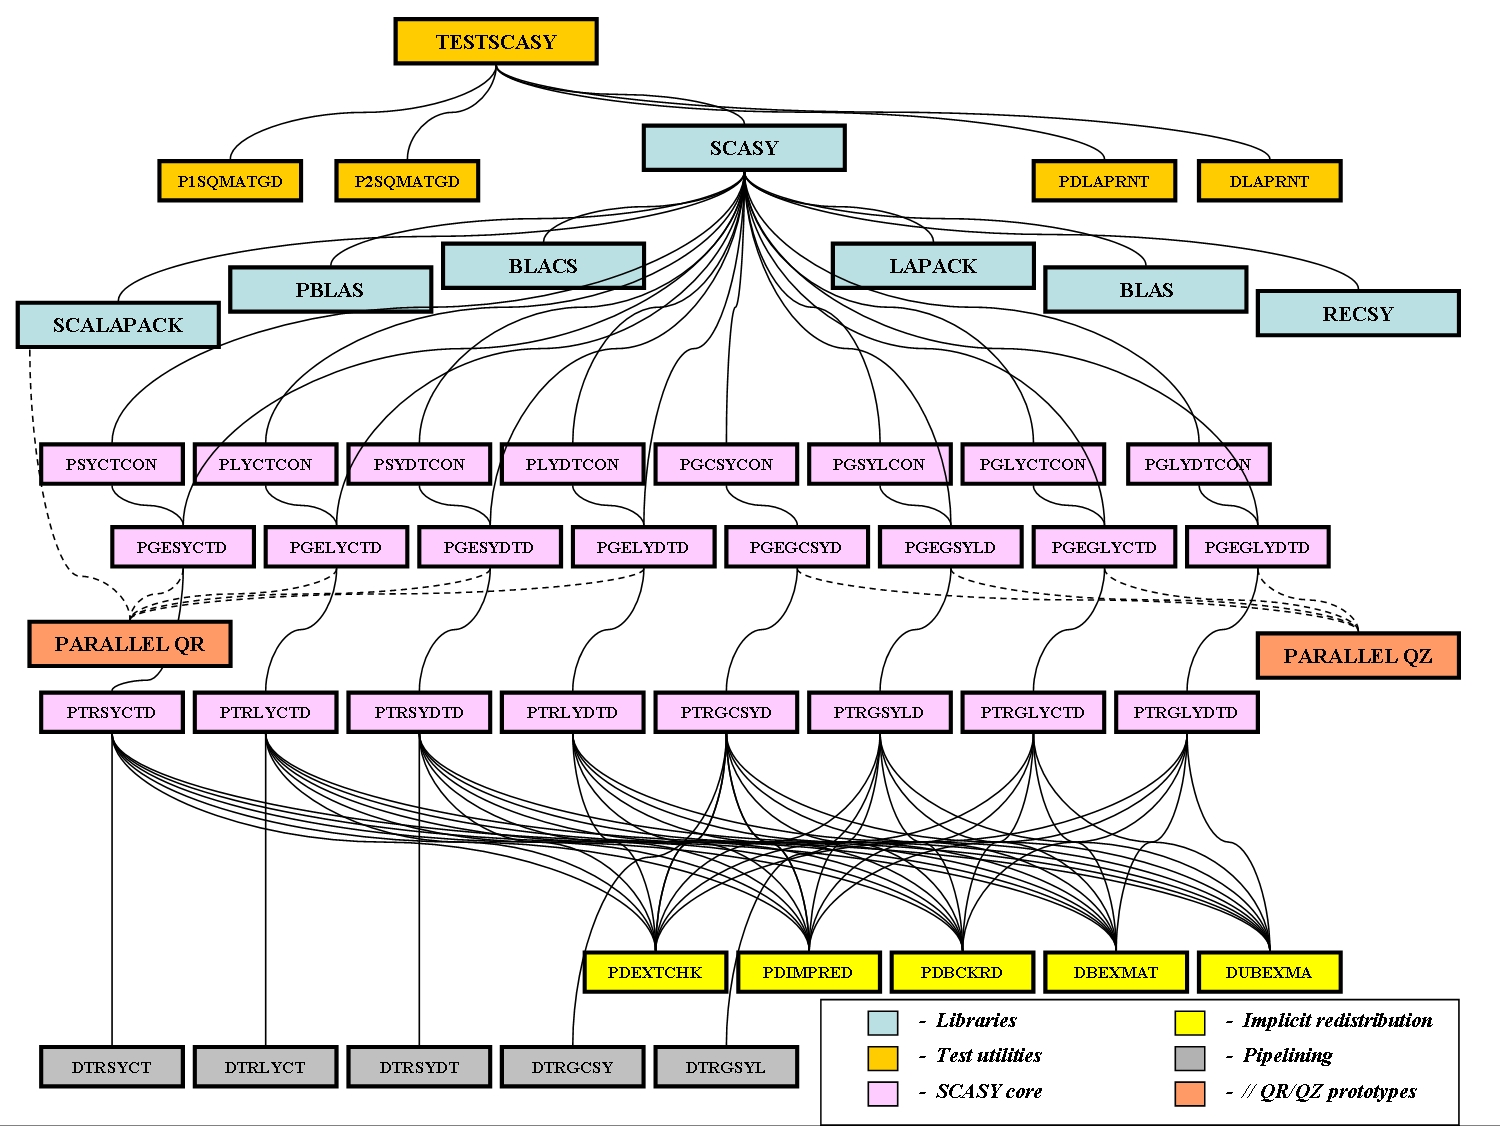
\includegraphics[scale=0.20]{scasy_callgraph.eps}
  \label{fig:callgraph}
\end{figure}
%
Below we give a glance of the internals of the SCASY software by 
presenting three types of the software in Figure \ref{fig:callgraph}: 
\emph{library dependencies}, \emph{parallel QR/QZ prototypes} and 
the routines used for performing \emph{implicit redistribution}.

\subsubsection{Libraries}
\label{sec:libraries} The following external libraries are used in
SCASY:
%
\begin{itemize}
    \item ScaLAPACK \cite{blackfordetal97,slug}
    including the PBLAS \cite{pblas} and BLACS \cite{blacs},
    \item LAPACK and BLAS \cite{lapack3},
    \item RECSY \cite{jonssonkagstrom03}, which provides almost
    all node solvers except for one transpose case of the GCSY
    equation. Notice that RECSY in turn calls a small
    set of subroutines from SLICOT ({\em Software Library in Control})
    \cite{slicot,slicotweb}.
\end{itemize}
%
For example, the routines for the standard matrix equations
utilize the ScaLAPACK routines \texttt{PDGEHRD}, which performs a
parallel Hessenberg reduction, \texttt{PDLAHQR}, which is the
parallel unsymmetric QR algorithm presented in
\cite{henrywatkinsdongarra02}, and \texttt{PDGEMM}, the PBLAS
parallel implementation of the level-3 BLAS GEMM-operation. The
triangular solvers employ the RECSY node solvers
\cite{jonssonkagstrom02a,jonssonkagstrom02b,jonssonkagstrom03} and
LAPACK's \texttt{DTGSYL} (see also \cite{kagstromporomaa96}) for
solving (small) matrix equations on the nodes and the BLAS for the
level 3 updates (\texttt{DGEMM}, \texttt{DTRMM} and
\texttt{DSYR2K} operations). To perform explicit communication and
coordination in the triangular solvers we use the BLACS library.

\subsubsection{Parallel QR/QZ prototypes} \label{sec:reductionproto}
The reduction to standard Schur form in the non-generalized matrix
equations are in the current release performed using existing
ScaLAPACK software. However, as pointed out and demonstrated in
\cite{granatkagstrom09a}, the current QR algorithm in ScaLAPACK
represents a time-consuming bottleneck of the reduction step in
the standard driver routines. A proposed revision of the parallel
QR algorithm with level 3 node performance and advanced deflation
techniques is presented in \cite{granatkagstromkressner09}.
Preliminary versions of these algorithms are attached to the
software package, and are accessed through wrappers to the existing
ScaLAPACK wrappers, provided the pre-processing option {\tt
USE\_NEWPQR} is defined on compile time (see also Section
\ref{sec:preprocess}). The following is the assumed Fortran
interface of the improved standard Schur reduction algorithm in
case of a direct call:

\begin{itemize}
\item \texttt{SUBROUTINE PDHSEQR( JOB, COMPZ, N, ILO, IHI, H,
DESCH, WR, WI, Z, DESCZ, \\ WORK, LWORK, IWORK, LIWORK, INFO )} \\
Computes the eigenvalues of the Hessenberg matrix $H$ and,
optionally, the matrices $T$ and $Z$ from the Schur decomposition
$T = Z^T H Z$, where $T$ is the Schur form and $Z$ is the
orthogonal matrix of Schur vectors.
\end{itemize}

The reduction of the involved matrix pairs to generalized real
Schur form is performed by linking with and invoking the new
prototype ScaLAPACK-style implementations of the
Hessenberg-triangular reduction and the parallel multi-shift QZ
algorithm presented in
\cite{adlerborndacklandkagstrom02,adlerbornkagstromkressner06}.
Presently, all associated QZ routines are provided as empty
wrappers which when invoked immediately return with the error code
{\tt INFO}=99, signalling that no computations were performed. The
following are the assumed Fortran interfaces of the generalized
Schur reduction algorithms:

\begin{itemize}
\item \texttt{SUBROUTINE PDGGHRD( COMPQ, COMPZ, N, ILO, IHI, A,
DESCA, B, DESCB, Q, \\ DESCQ, Z, DESCZ, WORK, LWORK, INFO )} \\
Computes the Hessenberg-triangular form $(H,T)$ by the orthogonal
equivalence transformation $(H,T) = Q^T(A,B)Z$, where the matrix
pair $(A,B)$ is regular and $B$ is assumed to be upper triangular
by an initial QR factorization.

\item \texttt{SUBROUTINE PDHGEQZ( JOB, COMPQ, COMPZ, N, ILO, IHI,
A, DESCA, B, DESCB, \\ ALPHAR, ALPHAI, BETA, Q, DESCQ, Z, DESCZ,
ILOQ, IHIQ, ILOZ, IHIZ, MXBLGS, \\ WORK, LWORK, INFO )} \\
Computes the generalized eigenvalues of the regular
Hessenberg-triangular matrix pair $(H,T)$ and, optionally, the
matrix pairs $(S,T)$ and $(Q,Z)$ from the generalized Schur
decomposition $(S,T) = Q^T(H,T) Z$, where $(S,T)$ is the
generalized Schur form and $Q$ and $Z$ are orthogonal matrices of
generalized Schur vectors.
\end{itemize}

These Schur reduction algorithms are still under development and
are not a part of the current SCASY contribution, which is
emphasized using dashes line in the subroutine hierarchy in Figure
\ref{fig:callgraph}. When production software for this software is
available they will be included in future SCASY releases. For an
explanation of the arguments of these Fortran interfaces, we refer
to the software documentation, which follows the standard
(Sca)LAPACK source documentation style.

\subsubsection{Implicit redistribution}
The handling of the implicit redistribution, caused by $2 \times
2$ diagonal blocks (corresponding to complex conjugate pairs
of eigenvalues), shared by multiple data layout blocks
(and processors) in the
left hand side quasi-triangular matrices of the matrix equations,
is concentrated to a few routines, as follows:
%
\begin{itemize}
    \item \texttt{PDEXTCHK} searches the diagonal
    blocks of a given matrix, say $A$, looking for any $2 \times 2$
    blocks shared by several data layout blocks. The routine returns the
    following {\em redistribution}
    information which decides which $\mbox{\em mb}_A \times \mbox{\em
    nb}_A$ diagonal blocks $A_{ii}$ that should be extended or diminished
    one row and column to include all elements of a shared $2 \times 2$
    block:
    \begin{displaymath}
        EXT\_INFO\_A(i) =
        \left\{ \begin{array}{ll}
        0 & \textrm{if $A_{ii}$ is unchanged} \\
        1 & \textrm{if $A_{ii}$ is extended} \\
        2 & \textrm{if $A_{ii}$ is diminished} \\
        3 & \textrm{if $A_{ii}$ is extended \emph{and} diminished}
        \end{array} \right. .
    \end{displaymath}
    This information is broadcasted to all processors and is used in
    \item \texttt{PDIMPRED}, in which data is exchanged between the
    processors via message passing to build up local arrays of extra elements which
    are used while constructing and decomposing the "correct"
    submatrices locally on the nodes by invoking the serial routines
    \texttt{DBEXMAT} and \texttt{DUBEXMA}.
    \item \texttt{PDBCKRD} is called right before returning from the
    corresponding triangular solver and sends back the
    redistributed parts of the solution matrix (pair) to their original
    owner processes such that the solution matrix (pair) is
    correctly distributed over the process mesh on output.
\end{itemize}
%
These routines are implemented in a general manner such that they
are easy to reuse in other applications involving distributed
quasi-triangular matrices.

\section{Terms of usage}
Any use of ACM Algorithms is subject to the ACM Software Copyright and 
License Agreement \cite{ACMsoftwarecrnotice}.
%The library is copyrighted and freely available for academic
%(non-commercial) use, and is provided on an "as is" basis. 
Moreover, use of the SCASY library should also be acknowledged by citing the
corresponding papers \cite{granatkagstrom09a,granatkagstrom09b}
and referring to the SCASY webpage \cite{scasy}.

\section{Conclusions and future work}
\label{sec:conclusions} We have presented the 1.0 release of the
high performance software library SCASY. The latest version of the
library along with updated information and documentation is always
available for download from the SCASY website \cite{scasy}. We
welcome bug-reports, comments and suggestions from users.

\section*{Acknowledgments}
The authors are grateful to the support staff of
HPC2N~\cite{hpc2n} for help with preparing the codes for this
release. \\

\noindent SCASY's main contributors are Robert Granat and Bo
K{\aa}gstr{\"{o}}m, Department of Computing Science and HPC2N,
Ume{\aa} University, Sweden. Collaborators and secondary
(indirect) contributors have been Bj{\"{o}}rn Adlerborn, Isak
Jonsson and Daniel Kressner.

{\small
\bibliographystyle{plain}
%\bibliography{allbib_090731}
\begin{thebibliography}{10}

\bibitem{ACMAlgPolicy}
{ACM TOMS Algorithms Policy}.
\newblock See \url{http://toms.acm.org/AlgPolicy.html}.

\bibitem{ACMsoftwarecrnotice}
{ACM Software Copyright and License Agreement}.
\newblock See \url{http://www.acm.org/publications/policies/softwarecrnotice}.

\bibitem{adlerborndacklandkagstrom02}
B.~Adlerborn, K.~Dackland, and B.~K\r{a}gstr\"om.
\newblock Parallel and blocked algorithms for reduction of a regular matrix
  pair to {H}essenberg-triangular and generalized {S}chur forms.
\newblock In J.~Fagerholm and et~al., editors, {\em Applied Parallel Computing
  PARA 2002}, volume 2367 of {\em Lecture Notes in Computer Science}, pages
  319--328. Springer-Verlag, 2002.

\bibitem{adlerbornkagstromkressner06}
B.~Adlerborn, B.~K\r{a}gstr\"om, and D.~Kressner.
\newblock {Parallel Variants of the Multishift QZ Algorithm with Advanced
  Deflation Techniques }.
\newblock In B.~K\r{a}gstr\"om et~al., editor, {\em Applied Parallel Computing:
  State of the Art in Scientific Computing, PARA 2006}, Lecture Notes in
  Computer Science, LNCS 4699, pages 117--126. Springer, 2007.

\bibitem{lapack3}
E.~Anderson, Z.~Bai, C.~Bischof, S.~Blackford, J.~W. Demmel, J.~J. Dongarra,
  J.~Du~Croz, A.~Greenbaum, S.~Hammarling, A.~McKenney, and D.~C. Sorensen.
\newblock {\em {LAPACK} Users' Guide}.
\newblock SIAM, Philadelphia, PA, third edition, 1999.

\bibitem{bartelsstewart72}
R.~H. Bartels and G.~W. Stewart.
\newblock {Algorithm 432: The Solution of the Matrix Equation {$AX - BX = C$}}.
\newblock {\em Communications of the ACM}, 8:820--826, 1972.

\bibitem{blackfordetal97}
L.~S. Blackford, J.~Choi, A.~Cleary, E.~D'Azevedo, J.~W. Demmel, I.~Dhillon,
  J.~J. Dongarra, S.~Hammarling, G.~Henry, A.~Petitet, K.~Stanley, D.~Walker,
  and R.~C. Whaley.
\newblock {\em {ScaLAPACK} Users' Guide}.
\newblock SIAM, Philadelphia, PA, 1997.

\bibitem{blacs}
{BLACS - Basic Linear Algebra Communication Subprograms}.
\newblock See \url{http://www.netlib.org/blacs/index.html}.

\bibitem{blanquer98parallelslicot}
I.~Blanquer, D.~Guerrero, V.~Hernandez, E.~Quintana-Orti, and P.~Ruiz.
\newblock {Parallel-SLICOT implementation and documentation standards}, 1998.

\bibitem{CALGO}
{Collected Algorithms of the ACM}.
\newblock See \url{http://calgo.acm.org}.

\bibitem{BLAS3a}
J.~J. Dongarra, J.~Du~Croz, I.~S. Duff, and S.~Hammarling.
\newblock A set of level 3 basic linear algebra subprograms.
\newblock {\em ACM Trans. Math. Software}, 16:1--17, 1990.

\bibitem{slicotweb}
E.~Elmroth, P.~Johansson, B.~K\r{a}gstr\"{o}m, and D.~Kressner.
\newblock A web computing environment for the {SLICOT} library.
\newblock In {\em The Third NICONET Workshop on Numerical Control Software},
  pages 53--61, 2001.

\bibitem{golubvanloan96}
G.~H. Golub and C.~F. Van~Loan.
\newblock {\em Matrix Computations}.
\newblock Johns Hopkins University Press, Baltimore, MD, third edition, 1996.

\bibitem{granatkagstrom07a}
R.~Granat and B.~K{\aa}gstr{\"{o}}m.
\newblock {Parallel Solvers for Sylvester-type Matrix Equations with
  Applications in Condition Estimation, Part I: Theory and Algorithms}.
\newblock Report {UMINF}-07.15, Dept. Computing Science, Ume{\aa} University,
  Sweden, 2007.
\newblock Revised August 2009.

\bibitem{granatkagstrom07b}
R.~Granat and B.~K{\aa}gstr{\"{o}}m.
\newblock {Parallel Solvers for Sylvester-type Matrix Equations with
  Applications in Condition Estimation, Part II: The SCASY Software}.
\newblock Report {UMINF}-07.16, Dept. Computing Science, Ume{\aa} University,
  Sweden, 2007.
\newblock Revised August 2009.

\bibitem{granatkagstrom09b}
R.~Granat and B.~K{\aa}gstr{\"{o}}m.
\newblock {ALGORITHM XXX: The SCASY Software Library -- Parallel Solvers for
  Sylvester-type Matrix Equations with Applications in Condition Estimation,
  Part II}.
\newblock 2009.
\newblock {\em {ACM} Transactions on Mathematical Software} (submitted July
  2007, revised January and August 2009, and March 2010).

\bibitem{granatkagstrom09a}
R.~Granat and B.~K{\aa}gstr{\"{o}}m.
\newblock {Parallel Solvers for Sylvester-type Matrix Equations with
  Applications in Condition Estimation, Part I: Theory and Algorithms}.
\newblock 2009.
\newblock {\em {ACM} Transactions on Mathematical Software} (submitted July
  2007, revised January and August 2009, and March 2010).

\bibitem{sug}
R.~Granat and B.~K{\aa}gstr{\"{o}}m.
\newblock {SCASY Users' Guide}.
\newblock Report {UMINF}-09.10, Dept. Computing Science, Ume{\aa} University,
  Sweden, 2010.

\bibitem{granatkagstromkressner09}
R.~Granat, B.~K{\aa}gstr{\"{o}}m, and D.~Kressner.
\newblock {A novel parallel QR algorithm for hybrid distributed memory HPC
  systems}.
\newblock {\em {\rm Submitted to} {SIAM Journal on Scientific Computing}},
  2009.
\newblock {From Technical report UMINF-09.06, also as LAPACK Working note
  \#216.}

\bibitem{granatkagstromporomaa03}
R.~Granat, B.~K{\aa}gstr{\"{o}}m, and P.~Poromaa.
\newblock {Parallel ScaLAPACK-style Algorithms for Solving Continuous-Time
  Sylvester Equations}.
\newblock In H.~Kosch and et~al, editors, {\em Euro-Par 2003 Parallel
  Processing}, volume 2790 of {\em Lecture Notes in Computer Science}, pages
  800--809. Springer, 2003.

\bibitem{hager84}
W.W. Hager.
\newblock Condition estimates.
\newblock {\em SIAM J. Sci. Statist. Comput.}, (3):311--316, 1984.

\bibitem{henrywatkinsdongarra02}
G.~Henry, D.~S. Watkins, and J.~J. Dongarra.
\newblock A parallel implementation of the nonsymmetric {QR} algorithm for
  distributed memory architectures.
\newblock {\em SIAM J. Sci. Comput.}, 24(1):284--311, 2002.

\bibitem{higham88}
N.~J. Higham.
\newblock Fortran codes for estimating the one-norm of a real or complex
  matrix, with applications to condition estimation.
\newblock {\em ACM Trans. of Math. Software}, 14(4):381--396, 1988.

\bibitem{hpc2n}
{HPC2N - High Performance Computing Center North}.
\newblock See \url{http://www.hpc2n.umu.se}.

\bibitem{jonssonkagstrom02a}
I.~Jonsson and B.~K{\aa}gstr{\"o}m.
\newblock {Recursive blocked algorithms for solving triangular systems. {Part
  I}. One-sided and coupled {S}ylvester-type matrix equations}.
\newblock {\em {ACM} Trans. Math. Software}, 28(4):392--415, 2002.

\bibitem{jonssonkagstrom02b}
I.~Jonsson and B.~K{\aa}gstr{\"o}m.
\newblock Recursive blocked algorithms for solving triangular systems. {Part
  II}. {T}wo-sided and generalized {S}ylvester and {L}yapunov matrix equations.
\newblock {\em ACM Trans. Math. Software}, 28(4):416--435, 2002.

\bibitem{jonssonkagstrom03}
I.~Jonsson and B.~K{\aa}gstr{\"{o}}m.
\newblock {RECSY - A High Performance Library for Solving Sylvester-Type Matrix
  Equations}.
\newblock In Kosch~H. et~al, editor, {\em {Euro-Par 2003 Parallel Processing}},
  volume 2790 of {\em Lecture Notes in Computer Science}, pages 810--819, 2003.

\bibitem{kagstromporomaa92}
B.~K{\aa}gstr{\"o}m and P.~Poromaa.
\newblock Distributed and shared memory block algorithms for the triangular
  {S}ylvester equation with {${\rm sep}\sp {-1}$} estimators.
\newblock {\em SIAM J. Matrix Anal. Appl.}, 13(1):90--101, 1992.

\bibitem{kagstromporomaa96}
B.~K{\aa}gstr{\"o}m and P.~Poromaa.
\newblock Computing eigenspaces with specified eigenvalues of a regular matrix
  pair {$(A,B)$} and condition estimation: theory, algorithms and software.
\newblock {\em Numer. Algorithms}, 12(3-4):369--407, 1996.

\bibitem{lapack}
{LAPACK - Linear Algebra Package}.
\newblock See \url{http://www.netlib.org/lapack/}.

\bibitem{pblas}
{PBLAS - Parallel Basic Linear Algebra Subprograms}.
\newblock See \url{http://www.netlib.org/scalapack/pblas}.

\bibitem{RECSY}
{RECSY - High Performance library for {S}ylvester-type matrix equations}.
\newblock See \url{http://www8.cs.umu.se/research/parallel/recsy}.

\bibitem{scasy}
{SCASY - ScaLAPACK-style solvers for {S}ylvester-type matrix equations}.
\newblock See \url{http://www8.cs.umu.se/research/parallel/scasy}.

\bibitem{slicot}
{SLICOT Library In The Numerics In Control Network (Niconet)}.
\newblock See \url{http://www.win.tue.nl/niconet/index.html}.

\bibitem{slug}
{ScaLAPACK Users' Guide}.
\newblock See \url{http://www.netlib.org/scalapack/slug/}.

\end{thebibliography}
}

\end{document}
